\documentclass[aspectratio=169,12pt]{beamer}

\usetheme{Madrid}
\usecolortheme{seahorse}
\setbeamertemplate{navigation symbols}{}
\setbeamertemplate{footline}[frame number]

\usepackage{amsmath,amssymb}
\usepackage{graphicx}
\usepackage{xcolor}
\usepackage{tikz}
\usetikzlibrary{arrows.meta,positioning}
\usepackage{listings}
\usepackage{booktabs}

\graphicspath{{../../plots/}}

\definecolor{topological}{HTML}{1f77b4}
\definecolor{critical}{HTML}{2ca02c}
\definecolor{trivial}{HTML}{d62728}
\definecolor{edgemode}{HTML}{e377c2}
\definecolor{codebg}{HTML}{f5f5f5}
\definecolor{codekw}{HTML}{0000cd}
\definecolor{codecomment}{HTML}{228b22}
\definecolor{codestring}{HTML}{8b0000}

\newcommand{\ket}[1]{|#1\rangle}
\newcommand{\bra}[1]{\langle#1|}
\newcommand{\Oedge}{X_0Z_1\cdots Z_{L-2}X_{L-1}}
\newcommand{\Tr}{\operatorname{Tr}}
\newcommand{\Pop}{\hat{P}}
\newcommand{\expv}[1]{\langle #1\rangle}

\title[Majorana Modes in the Machine]{Majorana Modes in the Machine}
\subtitle{Project Summary --- Kitaev Chain \& Majorana Zero Modes on NISQ Hardware}
\author{Dobromir Stoev\\ Edgar Harutyunyan\\ Guilherme Schewtschik\\ Jaskaran Singh\\ Zhengyi Liu\\ Zhenming Shi}
\institute{Advanced Seminar -- AI-Augmented Theoretical Physics}
\date{\today}

\begin{document}

\begin{frame}
  \titlepage
\end{frame}

% ---------------------------------------------------------------------------
\begin{frame}{The Project in One Slide}
  \begin{columns}[T]
    \begin{column}{0.55\textwidth}
      \small
      \textbf{The bridge: fermions $\to$ qubits $\to$ NISQ}
      \begin{itemize}
        \item The \textbf{1D Kitaev chain} is the minimal model of a 1D topological superconductor: in the topological phase it hosts \textbf{Majorana zero modes} localized at its two ends.
        \item A \textbf{Jordan--Wigner} map turns that fermionic model into an exact qubit Hamiltonian --- so a quantum device can, in principle, host the physics.
        \item We prepare its ground state by \textbf{VQE} and read the topological signature from a circuit-measurable observable.
      \end{itemize}
    \end{column}
    \begin{column}{0.45\textwidth}
      \small
      \begin{block}{The question}
        Can a \emph{topological signature} be prepared and still \emph{survive} on a noisy NISQ device --- and how far in system size $L$ can it be pushed?
      \end{block}
      \vspace{0.15cm}
      \footnotesize
      \textbf{Four Blocks:}
      \begin{enumerate}
        \item the physics bridge,
        \item finite-size physics \& qubit encoding,
        \item measuring topology with circuits,
        \item the NISQ reality check (results).
      \end{enumerate}
    \end{column}
  \end{columns}
\end{frame}

% ============================ BLOCK 1 =====================================
\begin{frame}{Block 1 --- The Physics Bridge}
  \begin{columns}[T]
    \begin{column}{0.52\textwidth}
      \centering
      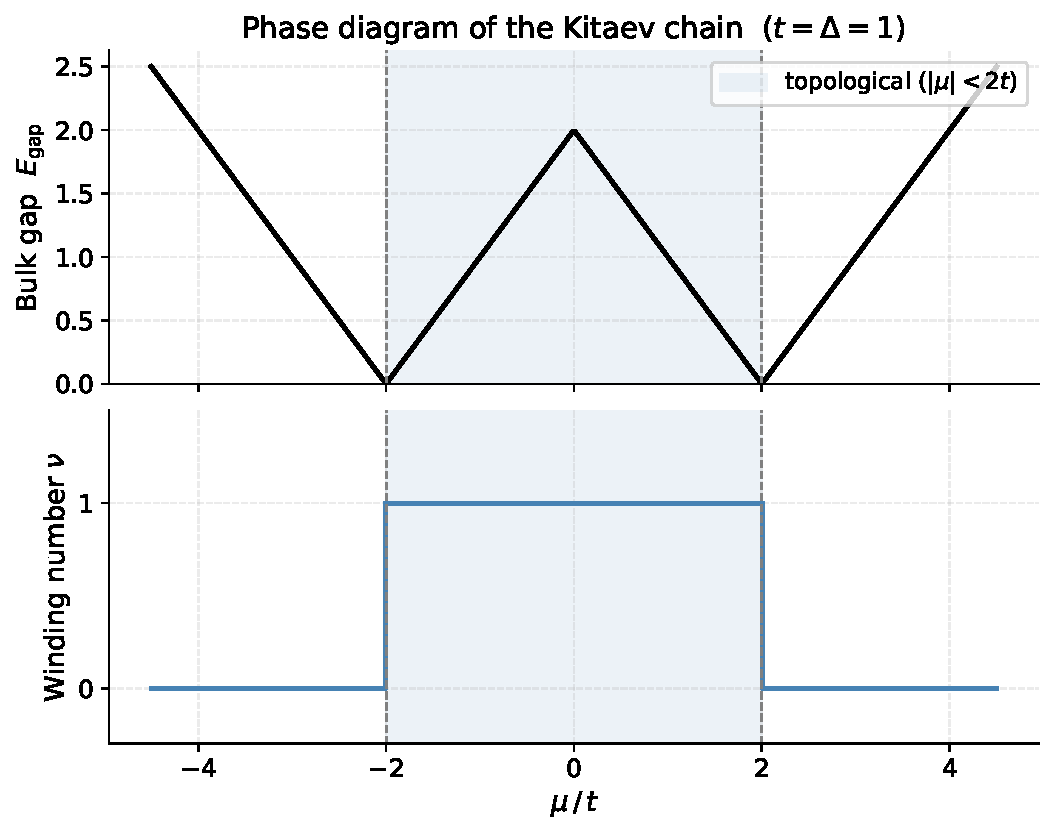
\includegraphics[width=\textwidth,height=0.72\textheight,keepaspectratio]{block1_03_phase_diagram.pdf}
    \end{column}
    \begin{column}{0.48\textwidth}
      \small
      The Kitaev chain: $p$-wave pairing on a 1D lattice,
      \[
        E_k=\sqrt{(\mu+2t\cos k)^2+(2\Delta\sin k)^2}.
      \]
      \begin{itemize}
        \item \textbf{Bulk gap} closes only at $|\mu|=2t$ --- the phase boundary.
        \item \textbf{Topological phase} for $|\mu|<2t$: a $\mathbb{Z}_2$ \textbf{winding number} $\nu=1$; trivial ($\nu=0$) outside.
        \item Bulk--boundary correspondence $\Rightarrow$ \textbf{Majorana zero modes} pinned to the ends in the topological phase.
      \end{itemize}
    \end{column}
  \end{columns}
\end{frame}

% ============================ BLOCK 2 =====================================
\begin{frame}{Block 2 --- Finite-Size Physics \& Qubit Encoding}
  \begin{columns}[T]
    \begin{column}{0.52\textwidth}
      \centering
      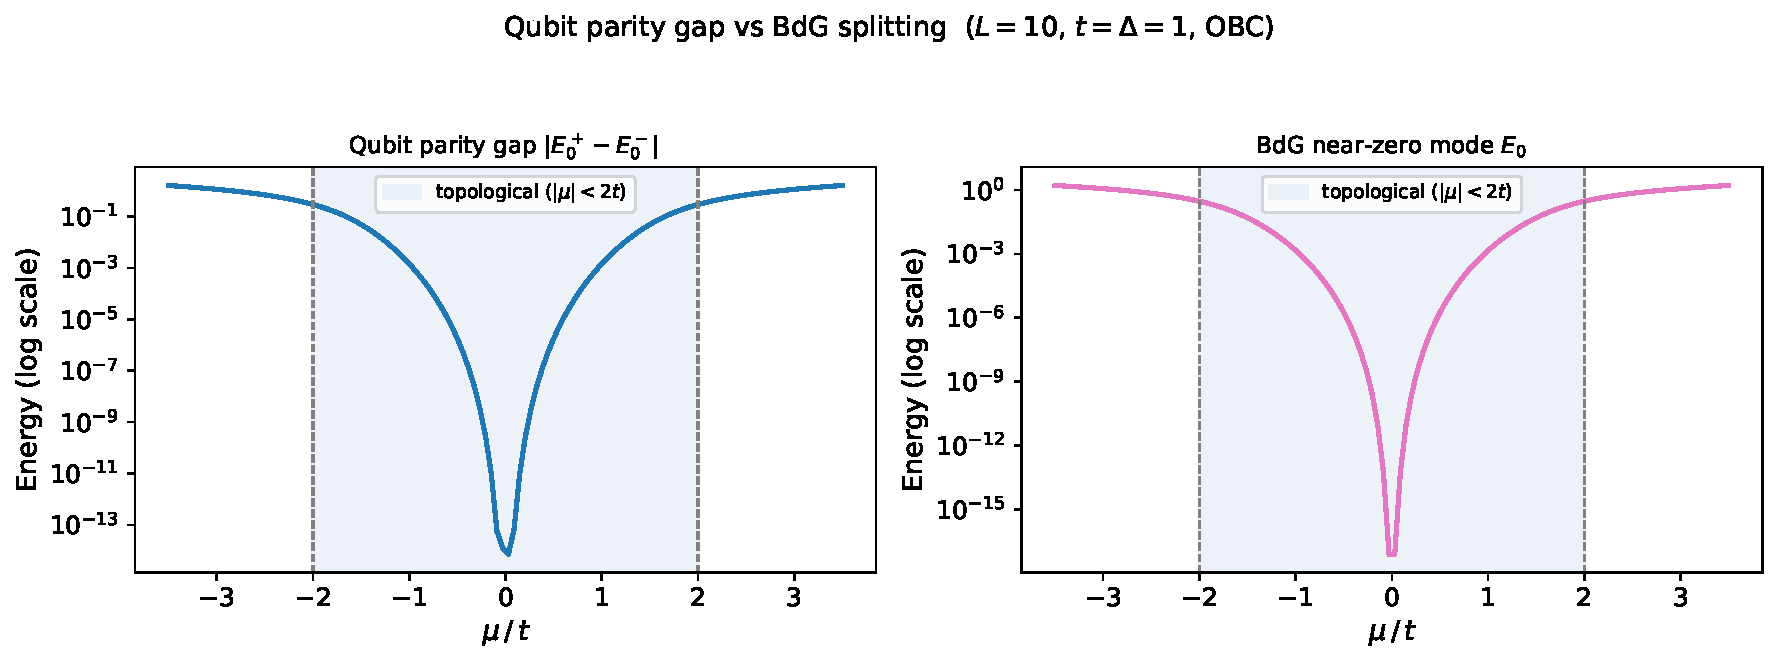
\includegraphics[width=\textwidth,height=0.72\textheight,keepaspectratio]{block2_01_parity_gap_vs_bdg.pdf}
    \end{column}
    \begin{column}{0.48\textwidth}
      \footnotesize
      On a finite chain the two end Majoranas overlap and split, $\Delta_P(L)\sim e^{-L/\xi}$.
      \begin{itemize}
        \item \textbf{Exponential protection}: the parity gap shrinks as the chain grows --- longer is better.
        \item \textbf{Jordan--Wigner} gives the \emph{exact} qubit Hamiltonian
        {\scriptsize\[
          H=-\tfrac{\mu}{2}\!\sum_j Z_j+\tfrac{t-\Delta}{2}\!\sum_j X_jX_{j+1}+\tfrac{t+\Delta}{2}\!\sum_j Y_jY_{j+1}.
        \]}
        \item \textbf{Parity} $\Pop=\prod_j Z_j$ is a $\mathbb{Z}_2$ symmetry: even/odd sectors label the two near-degenerate ground states.
      \end{itemize}
    \end{column}
  \end{columns}
\end{frame}

% ============================ BLOCK 3 =====================================
\begin{frame}{Block 3 --- Measuring Topology with Quantum Circuits (VQE)}
  \begin{columns}[T]
    \begin{column}{0.56\textwidth}
      \centering
      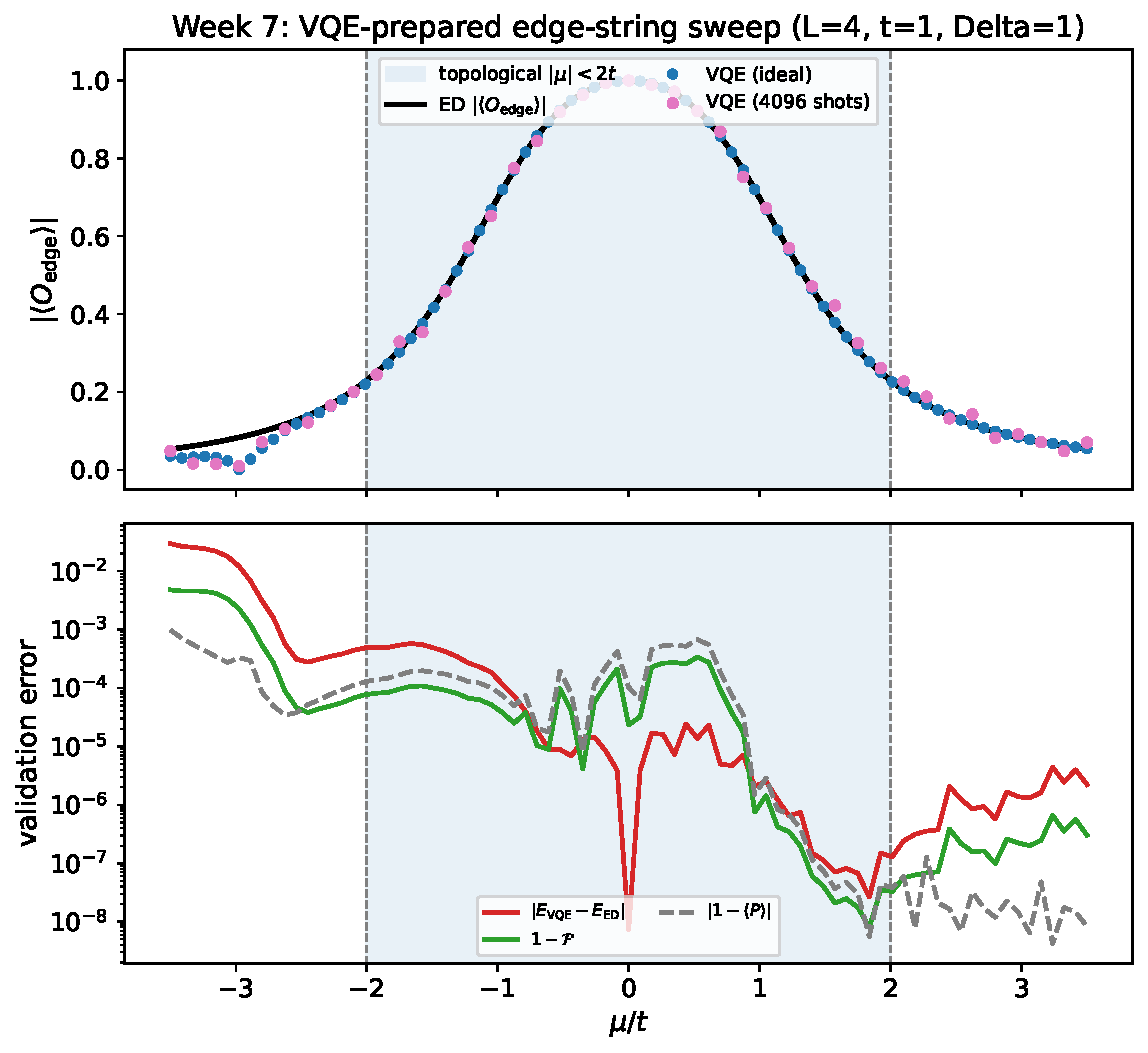
\includegraphics[width=\textwidth,height=0.72\textheight,keepaspectratio]{block3_week7_vqe_sweep.pdf}
    \end{column}
    \begin{column}{0.44\textwidth}
      \small
      Prepare the ground state \emph{variationally}, then detect the phase from a \emph{circuit-measurable} observable.
      \begin{itemize}
        \item \textbf{Parity-penalized VQE} (\texttt{EfficientSU2}) prepares the even-sector ground state --- no exact eigenvector needed.
        \item Topology lives in a \textbf{non-local edge string} $O_{\mathrm{edge}}=\Oedge$.
        \item Sweeping $\mu$: the string \textbf{turns on} in the topological phase, off in the trivial --- it tracks the transition.
      \end{itemize}
    \end{column}
  \end{columns}
\end{frame}

% ============================ BLOCK 4 =====================================
\begin{frame}{Block 4 --- NISQ Reality Check I: Noise Breaks the Diagnostic}
  \begin{columns}[T]
    \begin{column}{0.5\textwidth}
      \centering
      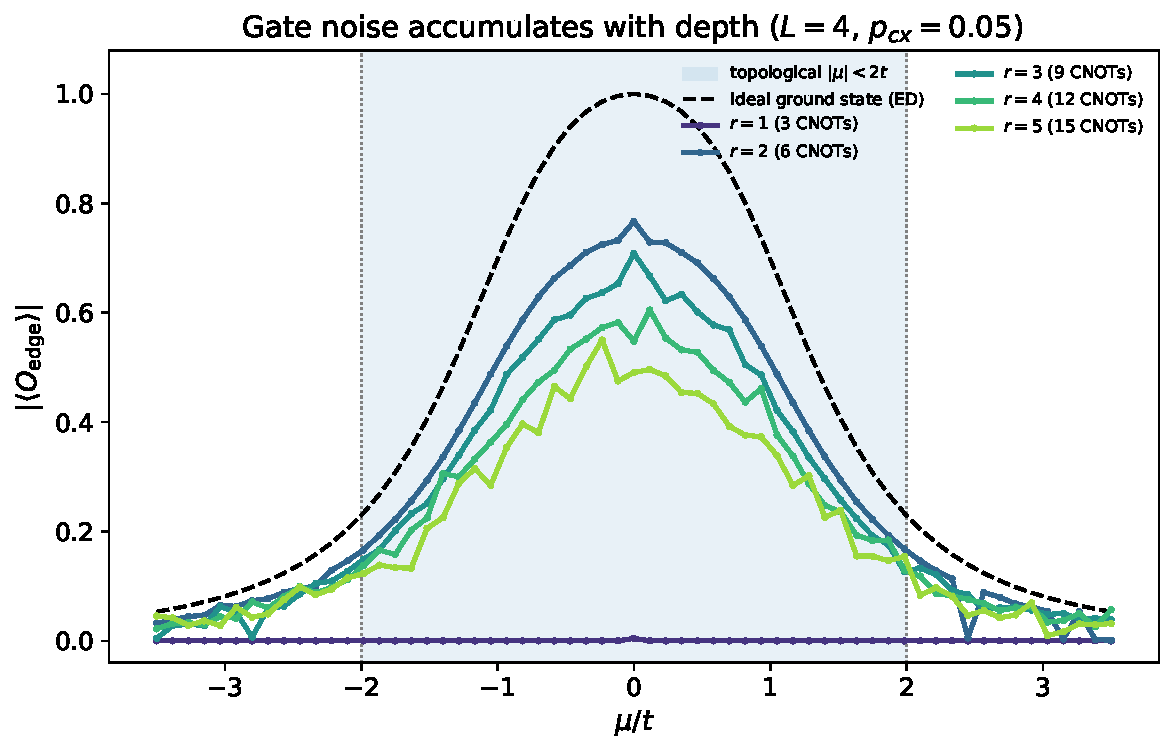
\includegraphics[width=\textwidth,height=0.62\textheight,keepaspectratio]{block4_week9_depth_sweep.pdf}
    \end{column}
    \begin{column}{0.5\textwidth}
      \centering
      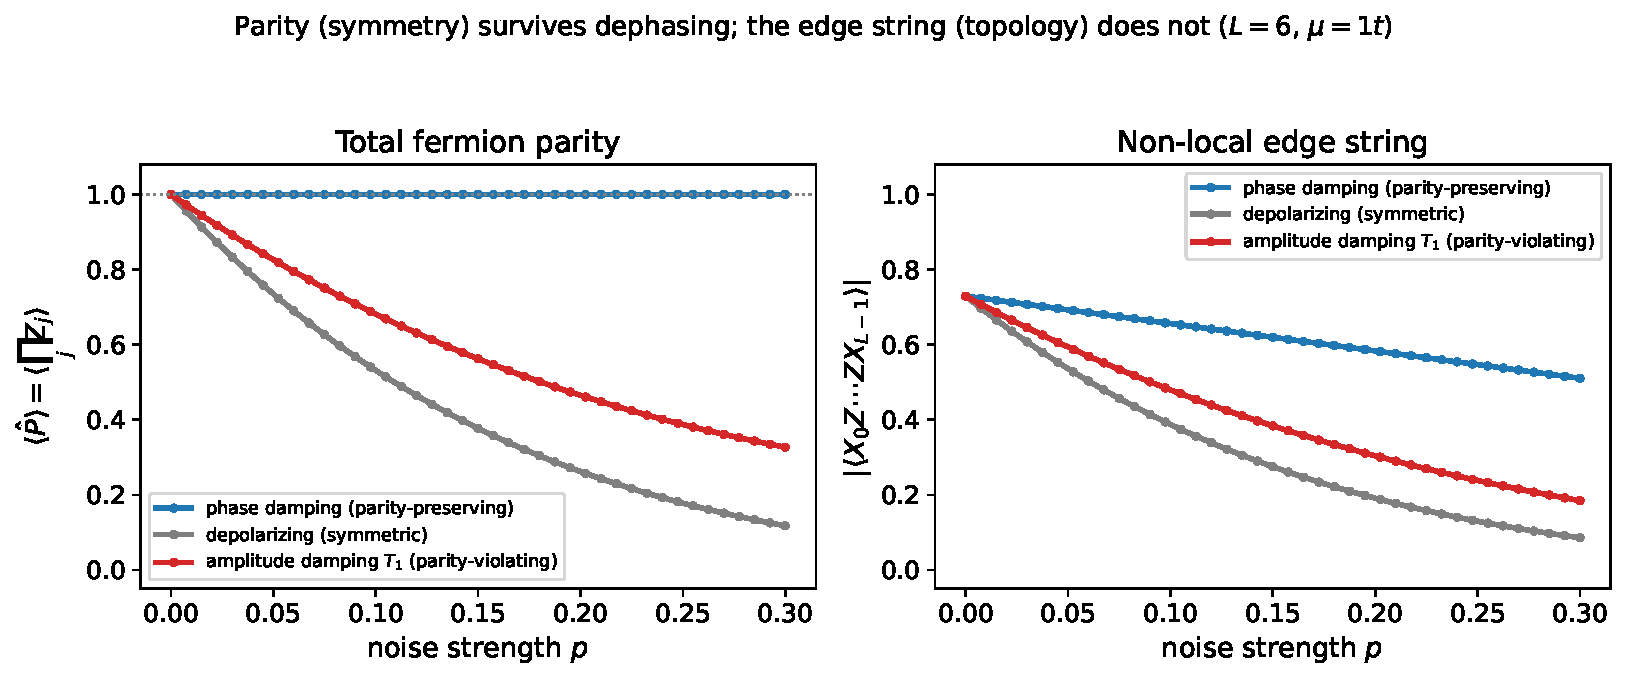
\includegraphics[width=\textwidth,height=0.62\textheight,keepaspectratio]{block4_parity_vs_noise.pdf}
    \end{column}
  \end{columns}
  \vspace{0.1cm}
  \footnotesize
  Circuit-level gate noise enters \emph{through the gates}: each \texttt{cx} adds an error channel, so the signal decays as $(1-p_{\mathrm{cx}})^{r(L-1)}$ with depth.
  \textbf{Left:} an under-expressive ansatz is dead everywhere; once expressive, deeper circuits are pushed down by accumulated CNOT noise.
  \textbf{Right:} \textcolor{topological}{parity is a symmetry} (protected under dephasing), but the \textcolor{trivial}{edge string (topology) is not noise-immune} --- it decays under every channel.
\end{frame}

\begin{frame}{Block 4 --- NISQ Reality Check II: Optimizing $\ne$ Preparing}
  \begin{columns}[T]
    \begin{column}{0.58\textwidth}
      \centering
      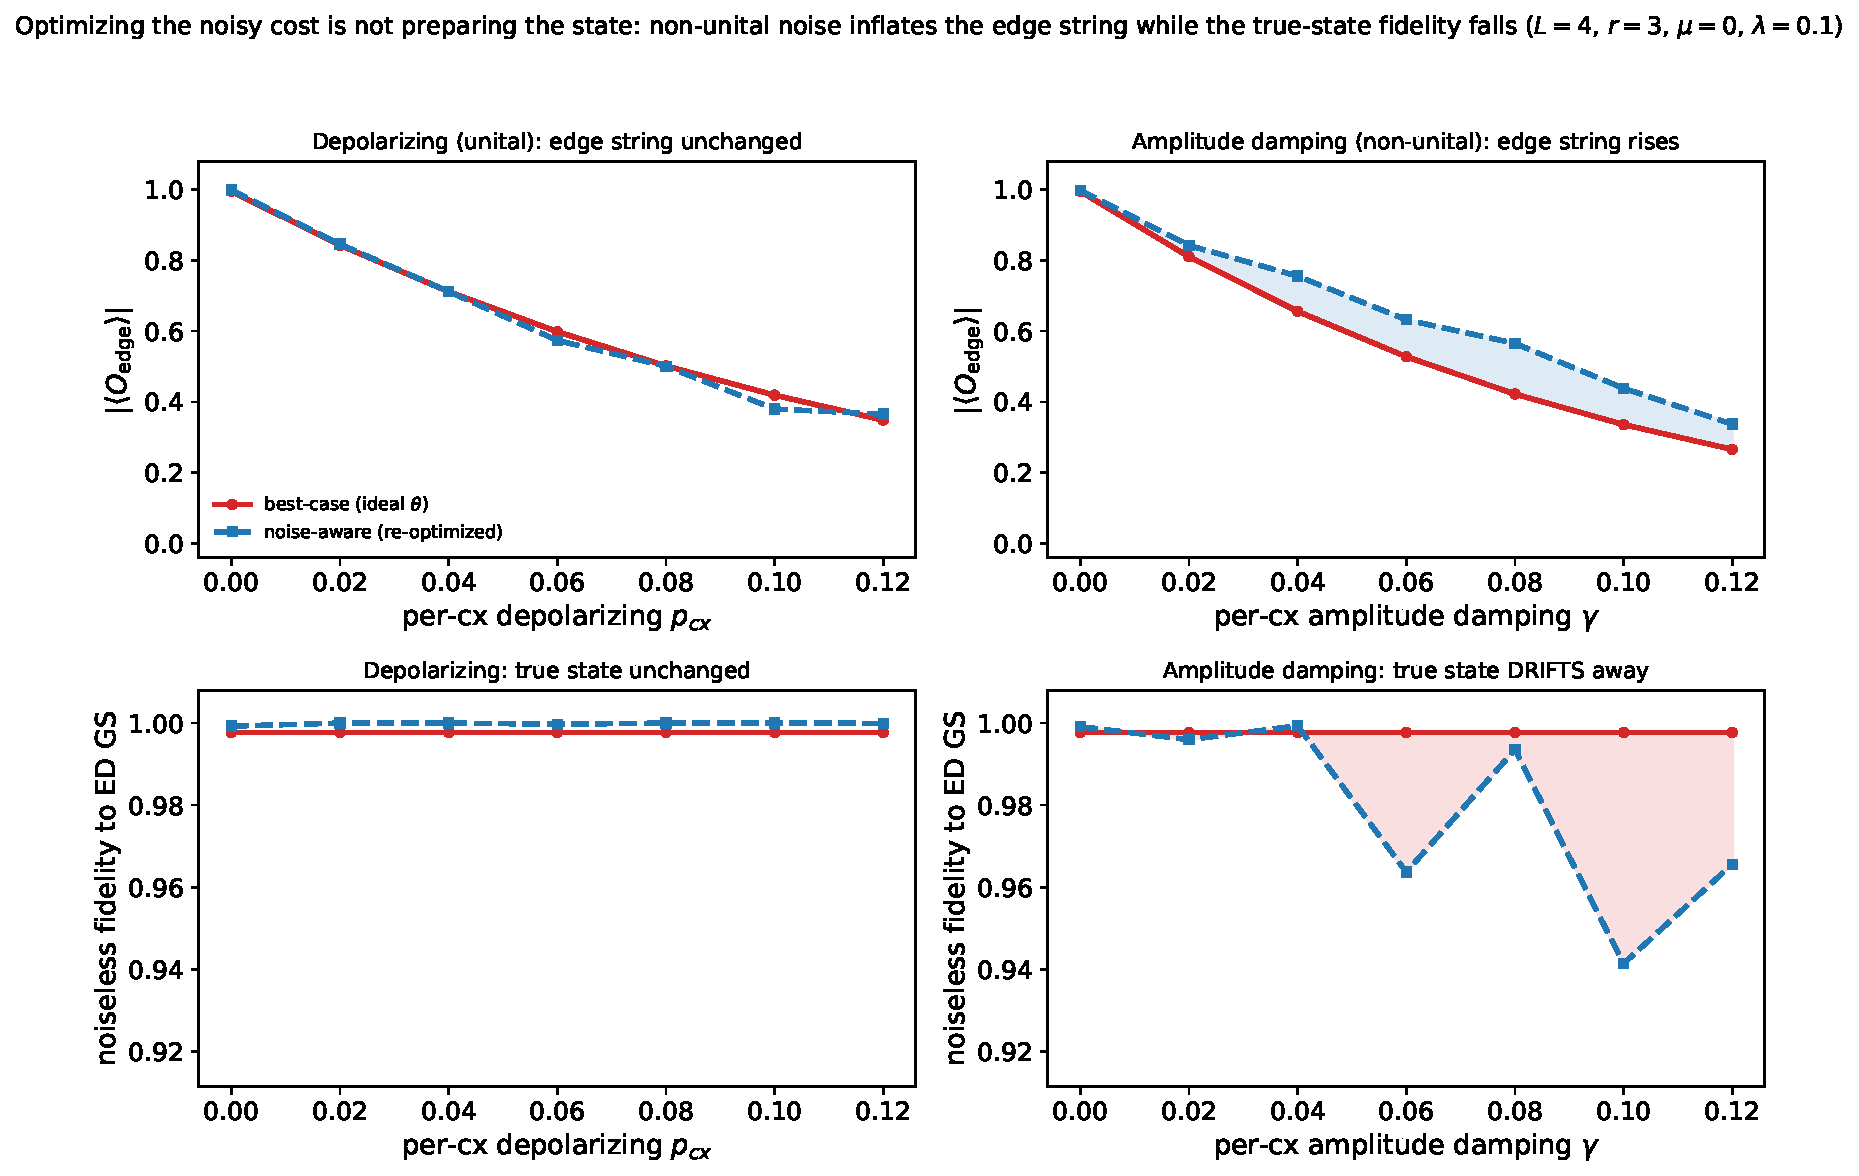
\includegraphics[width=\textwidth,height=0.74\textheight,keepaspectratio]{block4_week9_noisy_vqe.pdf}
    \end{column}
    \begin{column}{0.42\textwidth}
      \small
With a \texttt{NoiseModel}-backed estimator, \emph{every} VQE cost evaluation is corrupted.
      \begin{itemize}
        \item \textbf{The two rows:} \emph{top} $=$ measured edge string; \emph{bottom} $=$ \textbf{true-state fidelity} to the exact ground state.
        \item Non-unital noise ($T_1$, \emph{right}) \textbf{inflates the edge string} while \textbf{fidelity collapses} --- the observable lies.
        \item Optimizing the noisy cost $\ne$ preparing the state.
      \end{itemize}
    \end{column}
  \end{columns}
\end{frame}

\begin{frame}{Block 4 --- NISQ Reality Check III: Scaling to Large $L$ (Methods)}
  \small
  To push past the dense $L\!\approx\!15$ wall, the pipeline removes \emph{every} exponential object except the mild $2^L$ statevector.
  \begin{columns}[T,onlytextwidth]
    \begin{column}{0.47\textwidth}
      \begin{block}{Removing the two exponentials}
        \begin{itemize}
          \item \textbf{ED reference $\to$ free fermions}: the model is quadratic, so the exact ground state \& edge string come from a $2L\times2L$ \textbf{Bogoliubov--de~Gennes} matrix in $O(L^3)$.
          \item \textbf{$4^L$ density matrix $\to$ MPS trajectories}: the noisy edge string is sampled by \textbf{quantum-trajectory MPS} ($2^L$ per trajectory), $1/\sqrt{N}$ error bars.
        \end{itemize}
      \end{block}
    \end{column}
    \hfill
    \begin{column}{0.47\textwidth}
      \begin{block}{The mild object + HPC}
        \begin{itemize}
          \item \textbf{Ideal VQE}: a $2^L$ statevector with \emph{sparse} Pauli operators --- never the $4^L$ dense Hamiltonian ($\sim\!500\times$ faster at $L=14$).
          \item Working point $\mu=0.5t$ (gapped), L-BFGS-B optimizer, ED-free even-sector selection.
          \item The $(L,\text{reps})$ grid is parallelized on the \textbf{Leipzig SC cluster}.
        \end{itemize}
      \end{block}
    \end{column}
  \end{columns}
\end{frame}

\begin{frame}{Block 4 --- Methods Aside: MPS and the Bond Dimension $\chi$}
  \begin{columns}[T,onlytextwidth]
    \begin{column}{0.48\textwidth}
      \small
      \textbf{Matrix Product States (MPS)}
      \begin{itemize}
        \item An $L$-qubit state has $2^L$ amplitudes. An MPS factorizes that one giant tensor into a \textbf{chain of small per-site tensors} linked by \emph{virtual bonds}.
      \end{itemize}
      \vspace{0.15cm}
      \begin{center}
        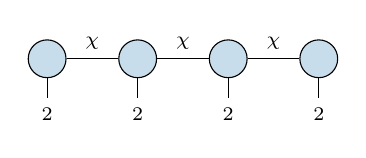
\begin{tikzpicture}[every node/.style={font=\scriptsize}]
          \foreach \x in {0,1,2,3} {
            \node[draw,circle,fill=topological!25,minimum size=0.48cm] (t\x) at (\x*1.15,0) {};
            \draw (t\x) -- ++(0,-0.5) node[below]{$2$};
          }
          \foreach \x/\y in {0/1,1/2,2/3} {
            \draw (t\x) -- (t\y) node[midway,above]{$\chi$};
          }
        \end{tikzpicture}
      \end{center}
      \vspace{0.1cm}
      Memory $2^L \to O(L\,\chi^2)$: \textbf{linear in $L$} whenever the bond dimension $\chi$ stays bounded.
    \end{column}
    \hfill
    \begin{column}{0.48\textwidth}
      \small
      \textbf{The bond dimension $\chi$}
      \begin{itemize}
        \item $\chi$ $=$ width of a virtual bond $=$ how much \textbf{entanglement} can cross a cut. Product state $\chi=1$; a generic (volume-law) state needs $\chi\sim2^{L/2}$.
        \item \textbf{Key:} our fixed-depth ansatz ($r$ reps of linear entanglers) builds at most $\chi\le 2^{r}$ across any cut --- set by \emph{circuit depth, not $L$}.
      \end{itemize}
      \vspace{0.1cm}
      At $r^\ast=4$: $\chi\le 16$ for \emph{every} $L$ --- the noisy edge string costs ${\sim}$linear in $L$, breaking the dense $L\!\approx\!15$ wall.
    \end{column}
  \end{columns}
\end{frame}

\begin{frame}{Block 4 --- NISQ Reality Check IV: The Scaling Result}
  \begin{columns}[T]
    \begin{column}{0.58\textwidth}
      \centering
      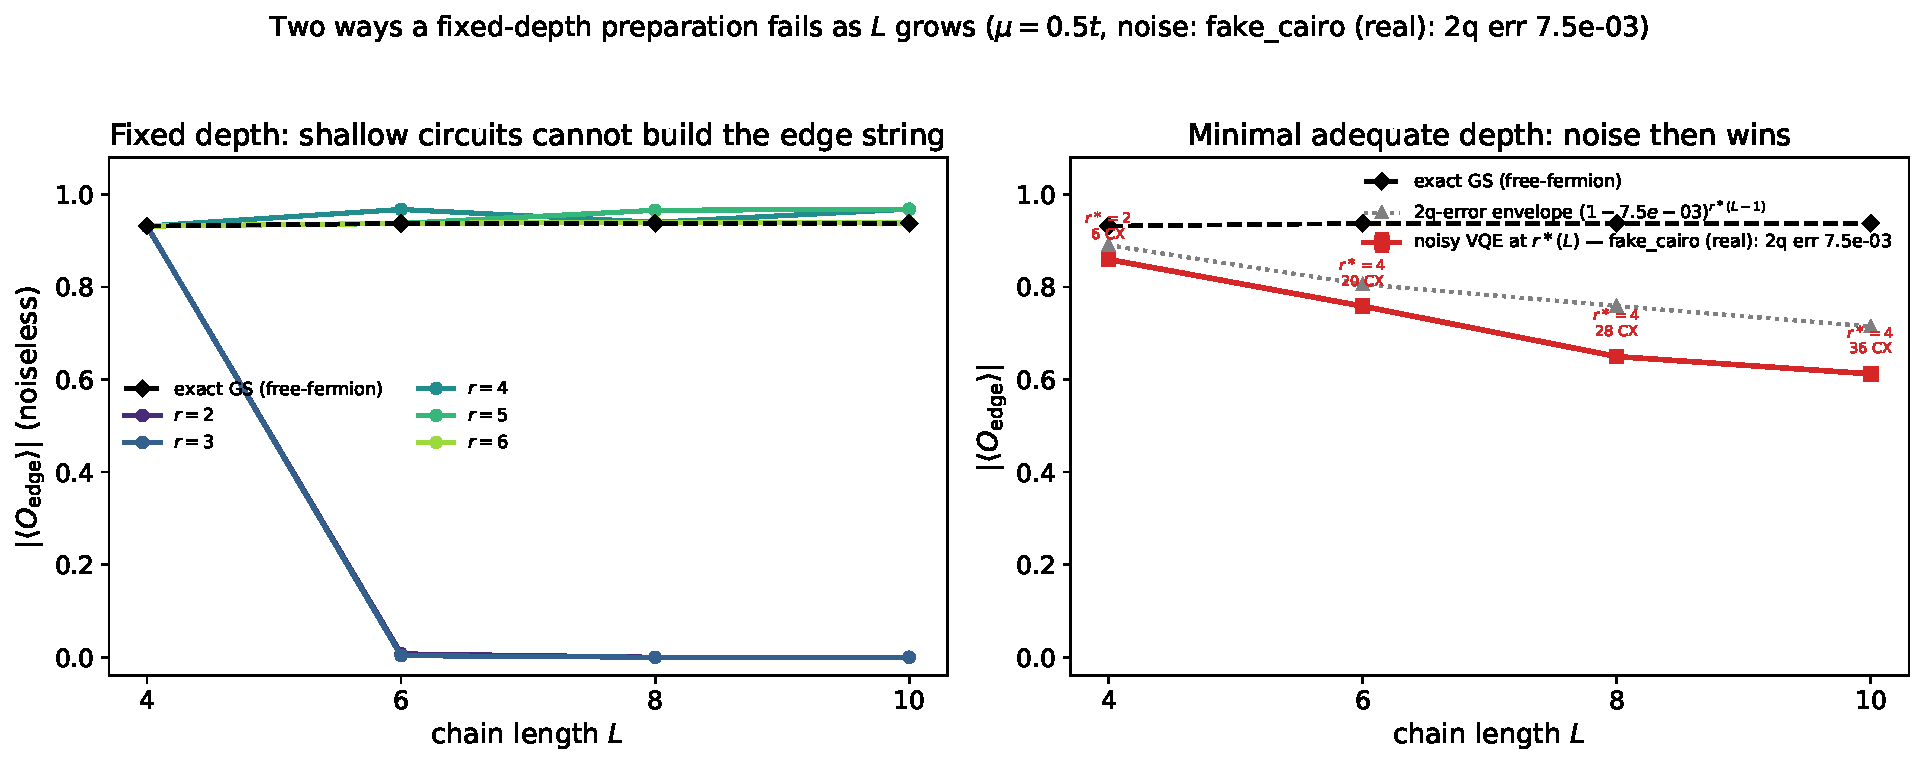
\includegraphics[width=\textwidth,height=0.72\textheight,keepaspectratio]{block4_scaling_Lsweep.pdf}
    \end{column}
    \begin{column}{0.42\textwidth}
      \small
      \textbf{The two failure modes decouple.}
      \begin{itemize}
        \item \textbf{Left:} expressibility is \emph{cheap and $L$-independent} --- a \textbf{constant} depth $r^\ast=4$ reproduces the edge string to $L=16$ (shallow $r=2,3$ fail).
        \item \textbf{Right:} at fixed depth $n_{\mathrm{cnot}}=4(L-1)$ grows \emph{linearly}, so \textbf{noise is the sole large-$L$ wall} --- the edge string decays exponentially.
      \end{itemize}
    \end{column}
  \end{columns}
  \vspace{0.05cm}
  \footnotesize
  Toy ($p=0.05$): dead by $L\!\approx\!14$. Real Cairo ($2q$ err ${\approx}0.0075$, ${\sim}6\times$ gentler) keeps $\expv{O_{\mathrm{edge}}}$ \emph{plateauing} ${\sim}0.5$ to $L=16$ --- it \textbf{survives far further} (next slide).
\end{frame}

\begin{frame}{Block 4 --- NISQ Reality Check V: Real Hardware to $L=100$}
  \begin{columns}[T]
    \begin{column}{0.62\textwidth}
      \centering
      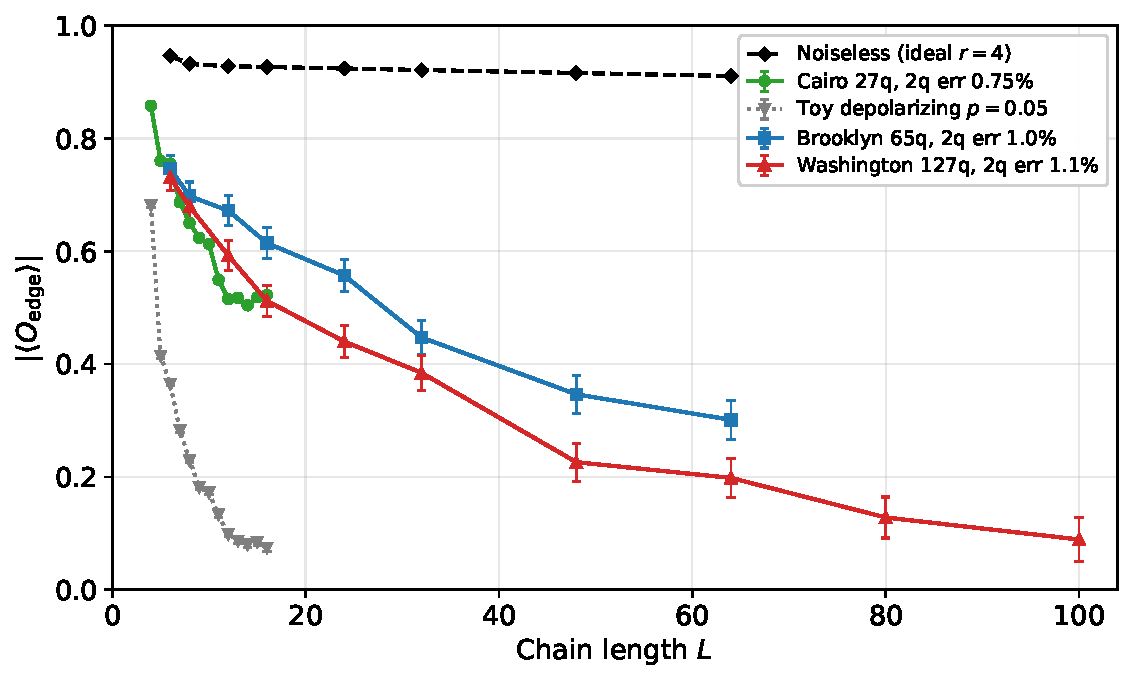
\includegraphics[width=\textwidth,height=0.80\textheight,keepaspectratio]{block4_largeL_overlay.pdf}
    \end{column}
    \begin{column}{0.38\textwidth}
      \small
      Every run at $r^\ast=4$, one axis.
      \begin{itemize}
        \item \textbf{Noiseless} (black): flat ${\sim}0.9$ --- topological at \emph{every} $L$.
        \item \textcolor{gray}{\textbf{Toy}} $p{=}0.05$: ${\sim}6\times$ too harsh, dead by $L=16$.
        \item \textbf{Real IBM} (\textcolor{critical}{Cairo} / \textcolor{topological}{Brooklyn} / \textcolor{trivial}{Washington}): survive far further; \textbf{agree on the overlap}, ordered by 2q error.
        \item Gone (${\sim}0.09$) only by $L=100$ --- decoherence over a \emph{linear} CNOT count.
      \end{itemize}
    \end{column}
  \end{columns}
\end{frame}

% ============================ CLOSING =====================================
\begin{frame}{Takeaways}
  \begin{itemize}
    \item The Kitaev chain's Majorana edge signature can be \textbf{prepared and measured on qubits} via a non-local string order $O_{\mathrm{edge}}=\Oedge$.
    \item \textbf{Parity (symmetry) is protected} under noise; the \textbf{edge string (topology) is not} noise-immune at fixed $L$.
    \item Classically, both exponentials are removable: the ED reference $\to$ \textbf{free fermions} (BdG), the $4^L$ density matrix $\to$ \textbf{MPS trajectories} --- only a mild $2^L$ statevector remains.
    \item For the edge-string diagnostic, \textbf{expressibility is $L$-independent} (constant depth $r^\ast=4$): the large-$L$ wall is \emph{decoherence} over a linearly growing gate count.
    \item On \textbf{real IBM noise} the signature \textbf{plateaus near ${\sim}0.5$} and stays measurable to $L=16$ --- far beyond where the toy model ($p=0.05$) predicts.
  \end{itemize}
  \vfill
  \centering
  \footnotesize Notes: \texttt{scaling\_to\_large\_L.tex}, \texttt{week9\_note.tex}, \texttt{parity\_topology\_protection.tex}.
\end{frame}

\end{document}
